\documentclass[activite]{thedocument}
\startdatakeys
\source{}
\cycle{}
\competencesDuSocle{}
\connaissancesRequises{}
\competencesTravaillees{}
\enddatakeys
\begin{document}
\begin{center}
    \LARGE LE JUNIPER GREEN
\end{center}
\vskip20pt
{\bfseries\Large Règles du jeu}
\begin{itemize}
    \item Le premier joueur coche un nombre sur la grille.
    \item Chaque joueur coche ensuite à son tour un nombre parmi les
    multiples ou les diviseurs du nombre choisi par son adversaire au
    coup précédent
    \item Lorsqu'un joueur ne peut plus jouer, son adversaire gagne la partie.
\end{itemize}
\vskip20pt
{\centering
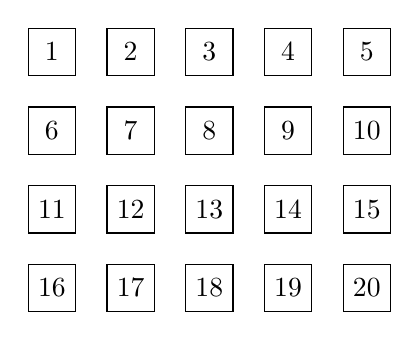
\begin{tikzpicture}
    \def\rectanglesize{0.3}
    \foreach\i in{0,1,...,3}{
        \foreach\j in{1,2,...,5}{
            \draw (\j-\rectanglesize,-\i-\rectanglesize)rectangle(\j+\rectanglesize,-\i+\rectanglesize);
            \draw node at(\j,-\i){\number\numexpr5*\i+\j};
        }
    }
\end{tikzpicture}\par}
\rule{\linewidth}{1pt}\vskip10pt
{\centering
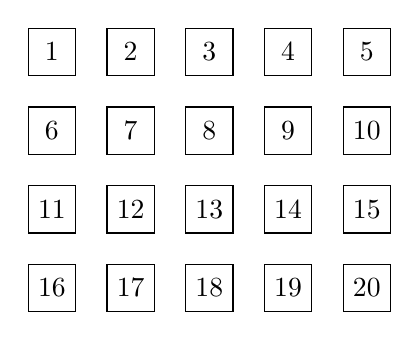
\begin{tikzpicture}
    \def\rectanglesize{0.3}
    \foreach\i in{0,1,...,3}{
        \foreach\j in{1,2,...,5}{
            \draw (\j-\rectanglesize,-\i-\rectanglesize)rectangle(\j+\rectanglesize,-\i+\rectanglesize);
            \draw node at(\j,-\i){\number\numexpr5*\i+\j};
        }
    }
\end{tikzpicture}\par}
\end{document}